\documentclass[12pt]{article}
\usepackage{fullpage}
\usepackage{graphicx, rotating, booktabs} 
\usepackage{times} 
\usepackage{fbb} 
\usepackage{natbib} 
\usepackage{indentfirst} 
\usepackage{setspace}
\usepackage{grffile} 
\usepackage{hyperref}
\usepackage{tikz-cd}
 \usetikzlibrary{cd}
\usepackage[export]{adjustbox}
\usepackage[most]{tcolorbox}
\usepackage{verbatimbox}
\usepackage{lscape}
\usepackage{afterpage}
\usepackage{amsmath}
\usepackage[labelfont={bf},textfont=it,labelsep=period]{caption}
 \usepackage{multirow} 
\setcitestyle{aysep{}}
\usepackage{dcolumn}

\hypersetup{
  colorlinks = true,
  urlcolor = blue,
  linkcolor = black,
  citecolor = black,
  pdfauthor = {Joshua Alley},
  pdfkeywords = {},
  pdftitle = {},
  pdfsubject = {},
  pdfpagemode = UseNone,
%  pdffitwindow = true
%  pdfcenterwindow = true
}



\singlespace
\title{\textbf{Alliances, Arms Exports and Electoral Trade Cycles}}
\author{Joshua Alley \\
Assistant Professor \\
University College Dublin\thanks{Thanks to Brian Blankenship, Jonathan Caverley, Jonathan Chu, Ben Fordham, Lauren Peritz, Erik Lin-Greenberg, Zachary Markovitch, Pieter Wezeman as well as participants in the Boston University Political Economy of Security Online Workshop Series and 2022 Meeting of the International Studies Association for helpful comments.} \\
joshua.alley@ucd.edu
}

 
\date{\today}

\bibliographystyle{apsr}

\usepackage{sectsty}
\sectionfont{\Large}
\subsectionfont{\noindent\large\textit}
\subsubsectionfont{\normalsize}

\makeatletter
\renewcommand\tiny{\@setfontsize\tiny{9}{10}}
\makeatother


\begin{document}

\maketitle 

\begin{abstract} 
Political budget cycles of defense contracting in the United States increase arms exports to allies, especially autocratic partners.  
When U.S. allies purchase weapons and accept arms transfers, they provide an outlet for outputs from efforts to use defense contracting to stimulate economic growth in key electoral areas.
Presidents and senators employ defense contracts because they have more control over this policy instrument than aggregate economic policy.
Alliance prot{\'e}g{\'e}'s positive economic and security statecraft thus helps U.S. leaders manipulate the economy during leadership competitions, and autocrats are especially able to accommodate electoral cycles.   
I examine these claims by analyzing the electoral determinants of defense contracting and arms export deals by the United States. 
First, I show how electoral concerns drive state-level contract awards with prime contracting data. 
I then detail corresponding electoral cycles in arms exports from the United States to allies. 
Third, I use a Bayesian model to link defense contract awards around elections directly to arms exports and then examines sectoral differences in weapons deals and contracting.
The results suggest that security and economic ties give political elites in alliance patrons additional tools to contest elections. 
\end{abstract} 


\newpage 
\doublespace 


\section{Introduction}


%% start with a good story of increased trade near elections: compare ally/not 
%% Matching for case selection produces: 1996 Denmark and Sweden
%U.S. trade with Denmark and Sweden spiked in 1996, as Bill Clinton ran for re-election.
%Exports to and imports from both Nordic countries rose, but Denmark received more U.S. exports.
%While these countries occupied similar regions and shared similar trade relations with the United States, Denmark received more exports because U.S. arms exports to this NATO member also rose.
%
%
%% give another example: Turkey and Egypt 1984
%Two Middle Eastern states experienced similar trade changes in 1984 when Ronald Reagan sought a second term.
%U.S. trade with Turkey and Egypt grew, but exports to Turkey increased more than exports to Egypt. 
%Like Denmark, Turkey had a formal U.S. security guarantee and thus received greater arms transfers and thus higher exports than Egypt, which did not have an alliance with the United States. 



% US-Brazil 1972
In 1972, the Nixon administration struck ten different deals to transfer or sell major conventional weapons to Brazil.
Among other systems Brazil's military dictatorship received 500 M-113 armoured personnel carriers, five destroyers, seven submarines, and eight S-2E Tracker anti-submarine warfare aircraft over the next four years.\footnote{All deal information from \citep{Sipri2022}.}
These deals came in a year when Richard Nixon sought reelection and continued after his 1974 resignation. 


% 
Similar events took place in 2012, when the Obama administration made twelve arms deals with Saudi Arabia. 
These deals included 400 Harpoon anti-ship missiles, 12 Apache attack helicopters for the Saudi National Guard, and 63 K-6 120mm mortars, along with parts for F-15 aircraft, other munitions, and other helicopters. 
Deliveries of these systems and other weapons spanned the next eight years, including the 2015 Saudi intervention in the Yemeni civil war. 





% example- PBC consequences vary w/ security coop
These instances reflect a more general pattern, where presidential elections in the United States expand arms exports to allies, especially autocratic states.
This paper unpacks the role of alliances and arms transfers in electoral trade cycles between the United States and other countries. 
I argue that U.S. allies receive more exports because they provide an easy outlet for arms transfers after defense contracting cycles. 


% arms exports logic
Security cooperation facilitates electoral cycles in arms exports. 
Leaders produce additional arms when they use defense contracting to create domestic political business cycles \citep{Tufte1978, Mintz1988, Mayer1995, DerouenHeo2000, Becker2021}.
Alliance prot{\'e}g{\'e}s provide a key market for exports from defense contracting cycles in part because leaders can easily justify transfers. 
Allies receive more arms from their patrons near elections because they control import decisions and receive security benefits. 
Autocratic allies are especially salient in this process because they receive more arms exports generally \citep{McManusYarhi-Milo2017}, and leaders face few constraints on accommodating electoral cycles.
These arms export cycles reinforce cooperative relationships between U.S. leaders and alliance prot{\'e}g{\'e}s.


Along with tracking defense contracting cycles, I examine the arms exports argument by showing that security factors do not modify electoral electoral trade cycles in imports.
In addition to defense contracting, elected leaders often use fiscal and monetary policy \citep{Nordhaus1975, Tufte1978, Rogoff1987, ClarkHallerberg2000} to boost economic growth around elections. 
Economic expansion from political business cycles in large states pulls in more imports.
Because foreign firms respond to increased domestic demand regardless of security relations, import cycles near elections serve as an important placebo check on the exports results.


% Findings
I scrutinize alliances, autocracy and arms export cycles in three ways. 
First, I show electoral cycles in contract awards in an analysis from 2000 to 2020.
I then demonstrate corresponding cycles in arms deals, where arms exports to allies rise as elections approach. 
Finally, I connect contracting and arms deals in a unified statistical model, and link contracts and arms deals within specific sectors.


% focus on the U.S.
The argument and analysis focus on the United States because it has the largest economy in the world, substantial alliance ties, and prior evidence of defense contracting cycles. 
Electoral arms transfer cycles will likely be weaker in other countries with smaller economies and defense industries. 
Still, the pivotal economic and security roles of the United States make understanding the economic and security consequences of U.S. political budget cycles worthwhile.
Furthermore, other cycles may occur in other states with different policy cycles. 


% economic and seucrity ties 
The argument and findings address three salient issues in international relations theory and practice. 
First, they detail the international consequences of political budget cycles. 
Domestic political business cycles in large countries like the United States reshape international economic exchanges and have knock-on effects in other countries \citep{Kayser2006, Kayser2009}.
Budget cycles also impact the international security environment. 


Second, I speak to a debate on economic and political leverage in asymmetric alliances like those between the United States and its partners falls. 
One argues that alliance patrons have limited economic leverage because they prioritize geopolitical aims \citep{Drezner2013, WolfordKim2017}.
Another perspective claims that alliance leaders have substantial economic influence \citep{Norrlof2010, Brooksetal2013} and threats to reduce security commitment encourage economic concessions \citep[pg. 122]{Oatley2015}.
Rather than analyze coercive economic demands, my argument explores how positive economic statecraft by allies helps U.S. leaders advance their electoral interests.


% coercion
Finally, this paper provides new insight into economic statecraft. 
Most economic statecraft scholarship studies economic sanctions (e.g. \cite{Marinov2005, Allen2008, Escriba-FolchWright2010}).
But as \citet{Baldwin2020} notes, economic statecraft includes positive inducements and negative sanctions. 
This paper examines positive economic statecraft--- how alliance prot{\'e}g{\'e} s use political economy decisions to indirectly facilitate patron leaders' political budget cycles.
As a result, it connects with prior work on issue linkage in alliance management, including studies of alliance formation \citep{Poast2012} and credibility \citep{Davis2008, Poast2013}. 


These claims also complement prior findings that foreign states use economic policies to manipulate electoral competition. 
\citet{KimMargalit2021} find that Chinese tariffs reduced Republican vote share in the 2018 midterm elections by targeting industries in competitive districts.
In the same way, \citet{ChyzhUrbatsch2021} find that Chinese soy tariffs hurt Republican congressional candidates in soy-producing areas. 
My argument inverts this logic by examining how security allies accommodate electoral budget cycles and help incumbents. 


% policy (THINK HARD ABOUT CUTTING)
Allied accommodation of political budget cycles by taking arms exports has important implications for alliance durability. 
Leaders who anticipate allied markets for outputs from defense contracting cycles will be more likely to demonstrate and uphold alliance commitment. 
Arms deal cycles are therefore a potential component of grand bargains between alliance patrons and their prot{\'e}g{\'e}s. 


% need an outline 
The paper proceeds as follows. 
To start, I outline an argument detailing the international consequences of political business cycles in the United States, the role of defense contracting in those cycles, and the consequences for arms deals. 
I then test the process in three steps. 
First, I establish the political business cycle roots of arms exports with evidence of defense contracting cycles. 
I then demonstrate that arms exports from the United States to allies increase more as presidential elections approach.
Third, I unify the preceding models with a joint Bayesian model of the process and link contracts with deals for specific weapons.
The last section discusses the results and offers concluding thoughts.


\section{Argument}


This argument explains how domestic political business cycles change the international arms trade. 
First, I detail constraints on aggregate budget cycle tools, which encourages U.S. elites to use defense contracting. 
I then discuss how presidential control and Congressional influence makes defense contracting an attractive policy tool for manipulating economic conditions around elections. 
After that, allies provide an market for outputs from electoral cycles in defense contracting. Among U.S. allies, autocracies with few constraints on their leaders and strong security motivations to curry favor by accepting arms are especially likely to make arms deals around elections.


Electoral considerations impact policy \citep{Nordhaus1975}.\footnote{See \citet{Dubois2016} for a review of the vast political budget cycle literature.} 
Leaders create political budget cycles by using fiscal and monetary policy to increase economic growth near elections and retain power for themselves or their party \citep{Tufte1978, Rogoff1987}. 
The composition and magnitude of these cycles varies. 
For example, strong central bank interdependence and fixed exchange rates make fiscal cycles more likely \citep{ClarkHallerberg2000}. 
%Even some independent central banks exhibit modest cyclical behavior, however \citep[pg. 247]{Dubois2016}


What tools leaders can use to bolster economic growth vary with national political institutions. 
Federal Reserve independence limits political influence on monetary policy in the United States, for instance.\footnote{Both Lyndon Johnson and Donald Trump found major limits to their ability to browbeat Federal Reserve Chairs into changing monetary policy. 
Johnson sought looser monetary policy before the 1968 presidential election, but Fed Chair William McChesney Martin continued to tighten policy.
Trump's tweeted demands for looser monetary policy to increase growth before the 2020 election similarly had little impact.}
Recent scholarship also highlights specific policy cycles because leaders struggle to manipulate aggregate economic instruments where they have more direct influence. 
In fiscal policy, aggregate budgets often give leaders limited spending discretion.


Limited flexibility with aggregate instruments encourages democratic leaders to use targeted policies to maximize the electoral impact of their limited discretion.
Some spending shifts can be more narrowly tailored \citep[pg. 248]{Dubois2016}.
Leaders also employ other policies such as trade disputes \citep{Conconietal2017}, labor agreements \citep{Ahlquist2010} and land reform \cite{Philips2020} to win support in key constituencies.


% Defense spending/contracts as flexible instrument
Scholars have long thought that defense spending is a useful instrument for budget cycles (e.g. \cite{Tufte1978, Mintz1988}).
Executive leaders often have more discretion in defense resource allocation, and defense spending has economic ramifications.
\citet{WhittenWilliams2011} note that defense spending can serve social welfare goals and \citet{Becker2021} finds that unemployment in NATO members encourages leaders to shift spending from equipment to personnel.


% in US context, contracts
Recent studies in the United States argue that defense budgets are poor political cycle tools, however, as Congress sets these levels two years ahead.
This shifted attention towards defense contracting, as leaders control contract timing and disbursement \citep{Mayer1995, DerouenHeo2000}.
Giving contracts also allows leaders to target key constituencies in response to unemployment and approval shifts by claiming credit for awards \citep{DerouenHeo2000}. 


% increased production of arms- not tied to security needs
Defense contracting increases arms production by employing firms to produce defense goods, and this has international consequences.\footnote{% Political Business cyles
Other work examines the international economic consequences of budget cycles.
Fiscal and monetary policy shifts impact currency prices and economic growth, which then alters trade and financial ties. 
Economic interdependence leads to correlated economic growth across countries \citep{ArtisZhang1999, Kayser2006} and increases the global economic influence of large economies. 
\citet{Ito1991} finds that U.S. elections increase economic growth in Japan, while \citet{ThompsonZuk1983} uncover some evidence of similar cycles in advanced industrial economies.
\citet{FoersterSchmitz1997} argue that U.S. electoral cycles impact international stock returns.
}
While these goods first equip the U.S. military, electoral cycles and defense planning may diverge.
Even the U.S. military may lack absorption capacity to incorporate defense contracting outputs.
Put differently, increased supply from electoral cycles in defense contracting does not respond to military demand, requiring other buyers. 
Foreign markets provide alternative outlets for new arms production from defense contracting cycles. 
When contracting cycles produce new goods, U.S. leaders can also sell or transfer old equipment to partners to make room.


% timeline and intermediate goods
These cycles are more likely to be evidence in arms export deals than deliveries. 
Production times for defense goods vary widely. 
Large platforms like ships, tanks and airplanes can take years to assemble. 
Still, if foreign states place orders for these platforms near elections, contracts can go out immediately.
Other goods such as small arms, ammunition and missiles, may be produced and exported more quickly. 
Intermediate goods, such as F-35 components, are also exported. 


% additional production and foreign markets
%When defense production and planning diverge, foreign markets provide alternative takers for excess arms production from defense contracting cycles. 
Not all countries are equally likely to make arms deals with the United States near elections, however. 
U.S. allies are more likely to take arms exports than other states. 
Security partners are a pivotal outlet because alliances facilitate security, economic and political cooperation.
The United States often transfers or sells arms to alliance prot{\'e}g{\'e} s, and these states have means and motivation to accommodate electoral cycles. 



\subsection{Alliances and U.S. Arms Exports}


% basic asymm alliance framework
In asymmetric alliances between large and small states, a larger patron protects a smaller prot{\'e}g{\'e}  in exchange for foreign policy concessions \citep{Morrow1991}.
A credible promise of military support increases the patron's foreign policy influence. 
Small alliance members garner protection from external threats and sacrifice some foreign policy autonomy. 


%Military alliances and economic cooperation are inseparable.
Many alliances also include explicit or implicit promises of economic cooperation \citep{GowaMansfield2004, LongLeeds2006, Davis2008, Poast2012}.\footnote{Conflict and economic integration are linked in general (see for example, \citep{GartzkeLi2003, Chen2021}).}
Prior research indicates that alliances promote trade \citep{Gowa1995, GowaMansfield2004, Haim2016} or protect existing trade ties \citep{Fordham2010}.
Alliances also encourage foreign direct investment \citep{LiVashchilko2010} and monetary cooperation \citep{Li2003}.
A cooperative bargain of security and economic cooperation results. 


% potential markets: allies
% take new or used stuff to make room
Bundled security and economic cooperation makes U.S. allies an obvious market for outputs from political cycles in defense contracting.\footnote{I focus here on formal and informal allies, because formal treaties like NATO are not the only areas with meaningful U.S. security commitments. Taiwan, Israel and Saudi Arabia have informal security guarantees, and often receive U.S. arms.}
\citet{Thurneretal2019} find that while the relative importance of security and economic factors fluctuates, alliances consistently increase arms transfers.
Common security interests and economic integration of defense industries create economic and security ties that encourage arms trade \citep{Bitzinger1994}. 
Defense industry integration generates trade in intermediate defense goods \citep{Brooks2005}. 


% less export cycles to non-allies
% each evidence sentence could be its own paragraph 
Allies are more likely than other states to receive arms around elections, and autocratic partners are especially likely to make arms deals. 
The security externalities of arms transfers constrain electoral cycles in arms exports to non-allies. 
U.S. elites will be less willing to increase the capability of states with fewer common interests, even if it facilitates electoral cycles.
Furthermore, arms transfers outside of alliances could face greater opposition scrutiny near elections, leading presidents to forestall criticism by forgoing contentious transfers.
Limited defense industry cooperation also constrains exports outside alliances to finished goods, while allies with defense industrial ties can receive intermediate goods.


% sending arms: political benefits for patron and prot{\'e}g{\'e} s
Moreover, electoral cycles in arms exports to allies benefit U.S. and allied leaders.
Presidents gain capacity to manipulate economic conditions with defense contracting and signal support for U.S. alliance prot{\'e}g{\'e} s by sending arms.
Defense contracting cycles increase prosperity in key electoral areas, which increases a leader's odds of winning office for themselves or their party.\footnote{\citet{Yarhi-Miloetal2016} argue that arms transfers sometimes substitute for formal alliances so patrons can provide security while managing entrapment risk.}

% positive statecraft tie-in from Baldwin 
Allied leaders also benefit from arms exports around elections, because arms exports curry favor with an alliance patron, bolster military capabilities and deepen perceived commitment.
Helping patron leaders by receiving arms will dispose the more favorably towards an ally. 
Allies increase their military capabilities with new arms as well, which can make their fighting forces more effective. 
Finally, because arms exports are a costly signal \citep{McManusYarhi-Milo2017}, allies gain confidence that their patron's commitment is credible. 


Allied leaders also have greater political freedom to make arms deals.
Arms imports are more flexible than tariffs or other trade policies that leaders could manipulate to boost trade with the United States.
Governments are the customer for most arms sales or transfers, so they have more latitude to take arms.
Direct control over these decisions mirrors how political control of firms increases trade policy flexibility \citep{Davisetal2019}.


Accepting arms exports is therefore positive economic and security statecraft by allies. 
Purchases and transfers are a common way that states bolster their political influence \citep[pg. 42-3]{Baldwin2020}.
In alliance politics, \citet[pg. 184-5]{IkenberryGrieco2003} note that states often use direct transfers to attract and sustain security commitments.  

% Sales and transfers- who pays for what
Moreover, prot{\'e}g{\'e} s do not always pay for U.S. arms.
The United States often subsidizes or gifts arms transfers through foreign military sales programs. 
While these still count as arms exports, they impose few immediate costs on recipients.
Alliances make such subsidized transfers to allies easier for presidents to justify to other elites, as they promote common security interests. 


\subsection{Autocratic Allies and Arms Deals}


While all allies might benefit from U.S. arms exports, autocratic allied leaders are more likely to make arms deals near elections. 
Autocracies have fewer domestic political constraints, which frees them to respond to U.S. defense contracting cycles.
They also have stronger security motivations to use arms deals to improve relations with the United States, because arms transfers are central to U.S. security guarantees to autocracies.


% constraints
Autocratic allies of the United States have greater political flexibility to make arms deals. 
Unlike democratic leaders who might face elite scrutiny of decisions to take additional U.S. arms, for example through legislative opposition, autocrats can strike a deal. 
Even if other domestic actors in an autocracy are opposed to additional outlays on U.S. arms, they have few ways to constrain the leader.\footnote{This changes when opponents of U.S. arms deals are part of the autocrats power base, but those bases are more narrow \citep{BDMetal2002}.}


% offstage signaling and need
Ability also meets need when autocrats take U.S. arms. 
The United States prefers ``offstage'' signals of support for autocrats, rather than public demonstrations of commitment \citep{McManusYarhi-Milo2017}.
Arms transfers are a pivotal signal of support in these relationships, and sometimes substitute entirely for formal security guarantees \citep{Yarhi-Miloetal2016}. 
When arms are the core of how the U.S. provides security, autocrats will be more willing to accept arms both to increase their military capabilities and signal continued alignment with the United States.


% further need- no ideological affinity
Autocrats are also limited in their ability to use other tools to curry favor with U.S. leaders.
Formal alliances might promote democratization \citep{GiblerWolford2006, Warren2016}.
The U.S. public is less likely to approve of alliances with an autocrat \citep{Alley2022}, so autocrats may also have little freedom to pursue deeper ties in other areas. 
The net result is that arms deals are central to U.S. ties with autocratic security partners, so autocrats are more likely to make arms deals when defense contracting cycles make it more likely. 



% deliberate or not?- key for statecraft argument. 
This argument is agnostic about whether allies make a conscious decision to help political budget cycles by taking arms exports.
While they want improve their alliance relationship, U.S. allies need not choose to accommodate electoral cycles in defense contracting.
Allies may receive better terms and more financial support to take additional goods, or take transfers or surplus materiel as a deliberate favor to leaders who have supported their foreign policy interests. 


The overall argument process is as follows.
First, budget cycles increase defense contracting awards. 
As defense contracting increases arms production, increased arms exports to allies follow. 
\autoref{fig:arg-process} summarizes this sequence.


\begin{figure}[htpb]
\adjustbox{scale = .85}{
\centering
\begin{tikzcd}[ampersand replacement=\&]
\mbox{Electoral Budget Cycles} \arrow[r]  \& \mbox{Defense Contracting} \arrow[r] \& \mbox{Arms Production} \arrow[r] \& \mbox{Arms to Autocratic Allies}
\end{tikzcd}
}
\caption{Summary of the argument process linking budget cycles in defense contracting to electoral cycles in U.S. arms deals.}
\label{fig:arg-process}
\end{figure}


%\begin{table}
%\resizebox{.99\textwidth}{!}{
%\begin{tabular}{ccccccc}
%\mbox{Budget}  & $\rightarrow$    & \mbox{Defense}     & $\rightarrow$ & \mbox{Arms}     & $\rightarrow$ & \mbox{Trade Cycles, especially} \\
%\mbox{Cycles}  &                  & \mbox{Contracting} &               &  \mbox{Production}   &               & \mbox{Arms to Allies} \\
%\end{tabular}
%}
%\end{table}


% Result- increased exports, tied to electoral cycles
The result of this process is more arms deals as elections approach, especially with autocratic alliance prot{\'e}g{\'e}s.
Arms exports in turn are rooted in electoral cycles of defense contracting.



\subsection{Implications}



The argument generates several testable implications within specific scope conditions. 
Cycles are most likely in states with a significant domestic defense industry and many security commitments.
Fixed election scheduling further reduces endogeneity between policy decisions and election timing.
Therefore, the argument and analysis focus on the United States. 
Other states may have weaker cycles, or electoral cycles in different goods.


The first prediction tests the expected relationship between defense contracts and arms exports. 
I expect electoral cycles in defense contacting, and a positive correlation between these cycles and U.S. arms exports.


\begin{quote}
\textsc{Defense Contracts Hypothesis: As electoral competition in a state increases, prime defense contract awards increase.}
\end{quote}


The second hypothesis predicts corresponding cycles in arms exports, especially to autocratic allies.
Proximity to presidential elections will increase arms transfers from the United States to autocratic allied states. 


\begin{quote}
\textsc{Arms Exports Hypothesis: As time to a presidential election decreases, U.S. arms exports to autocratic allies will increase.}
\end{quote}




% What's next
In the following, I examine each of these hypotheses. 
In the first analysis, I use a series of descriptive data and single-outcome statistical models to illustrate each step in the process.
This starts with descriptive data on defense contracting from 2000 to 2020, then shows how arms exports to allies track U.S. electoral cycles, and ends with a model of electoral cycles in U.S. trade. 
After that, I unify the different outcomes in Bayesian model that captures the process where contract allocations to electorally important states filter up into arms exports, ultimately driving increased exports.


\section{Defense Contracting Cycles}


To show electoral cycles in defense contracting, I draw on Department of Defense prime contract award data from the USAspending.gov database.\footnote{Link here: \url{https://www.usaspending.gov/download_center/custom_award_data}.} 
This archive contains data on individual contract awards starting in the 2000 fiscal year, and I collected all Department of Defense contracts from 2000 to 2020.


In addition to aggregating the total federal dollar obligation of all contracts in every year, I differentiate contracts by sector to assess which sectors drive contracting cycles. 
I measure total contracts for aircraft, ships, vehicles, electronics, missiles/space, and weapons/ammunition. 
While large contracts for components of major combat platforms have greater economic heft, full platforms can take years to deliver. 
Missiles, weapons and ammunition may lead to more immediate exports of defense goods, as their production schedules are more flexible.


If defense contracting drives electoral export cycles, we should observe electoral cycles in defense contracting.
\autoref{fig:contract-cycles} shows defense contracting cycles around presidential elections. 
As presidential elections approach, aggregate defense contract awards increase. 
There is a notable spike of \$25-30 billion in the median of overall defense contracts from two years into a presidential term to one year before an election. 
Median defense contracting levels rise further in election years.


\begin{figure}[htpb]
	\centering
		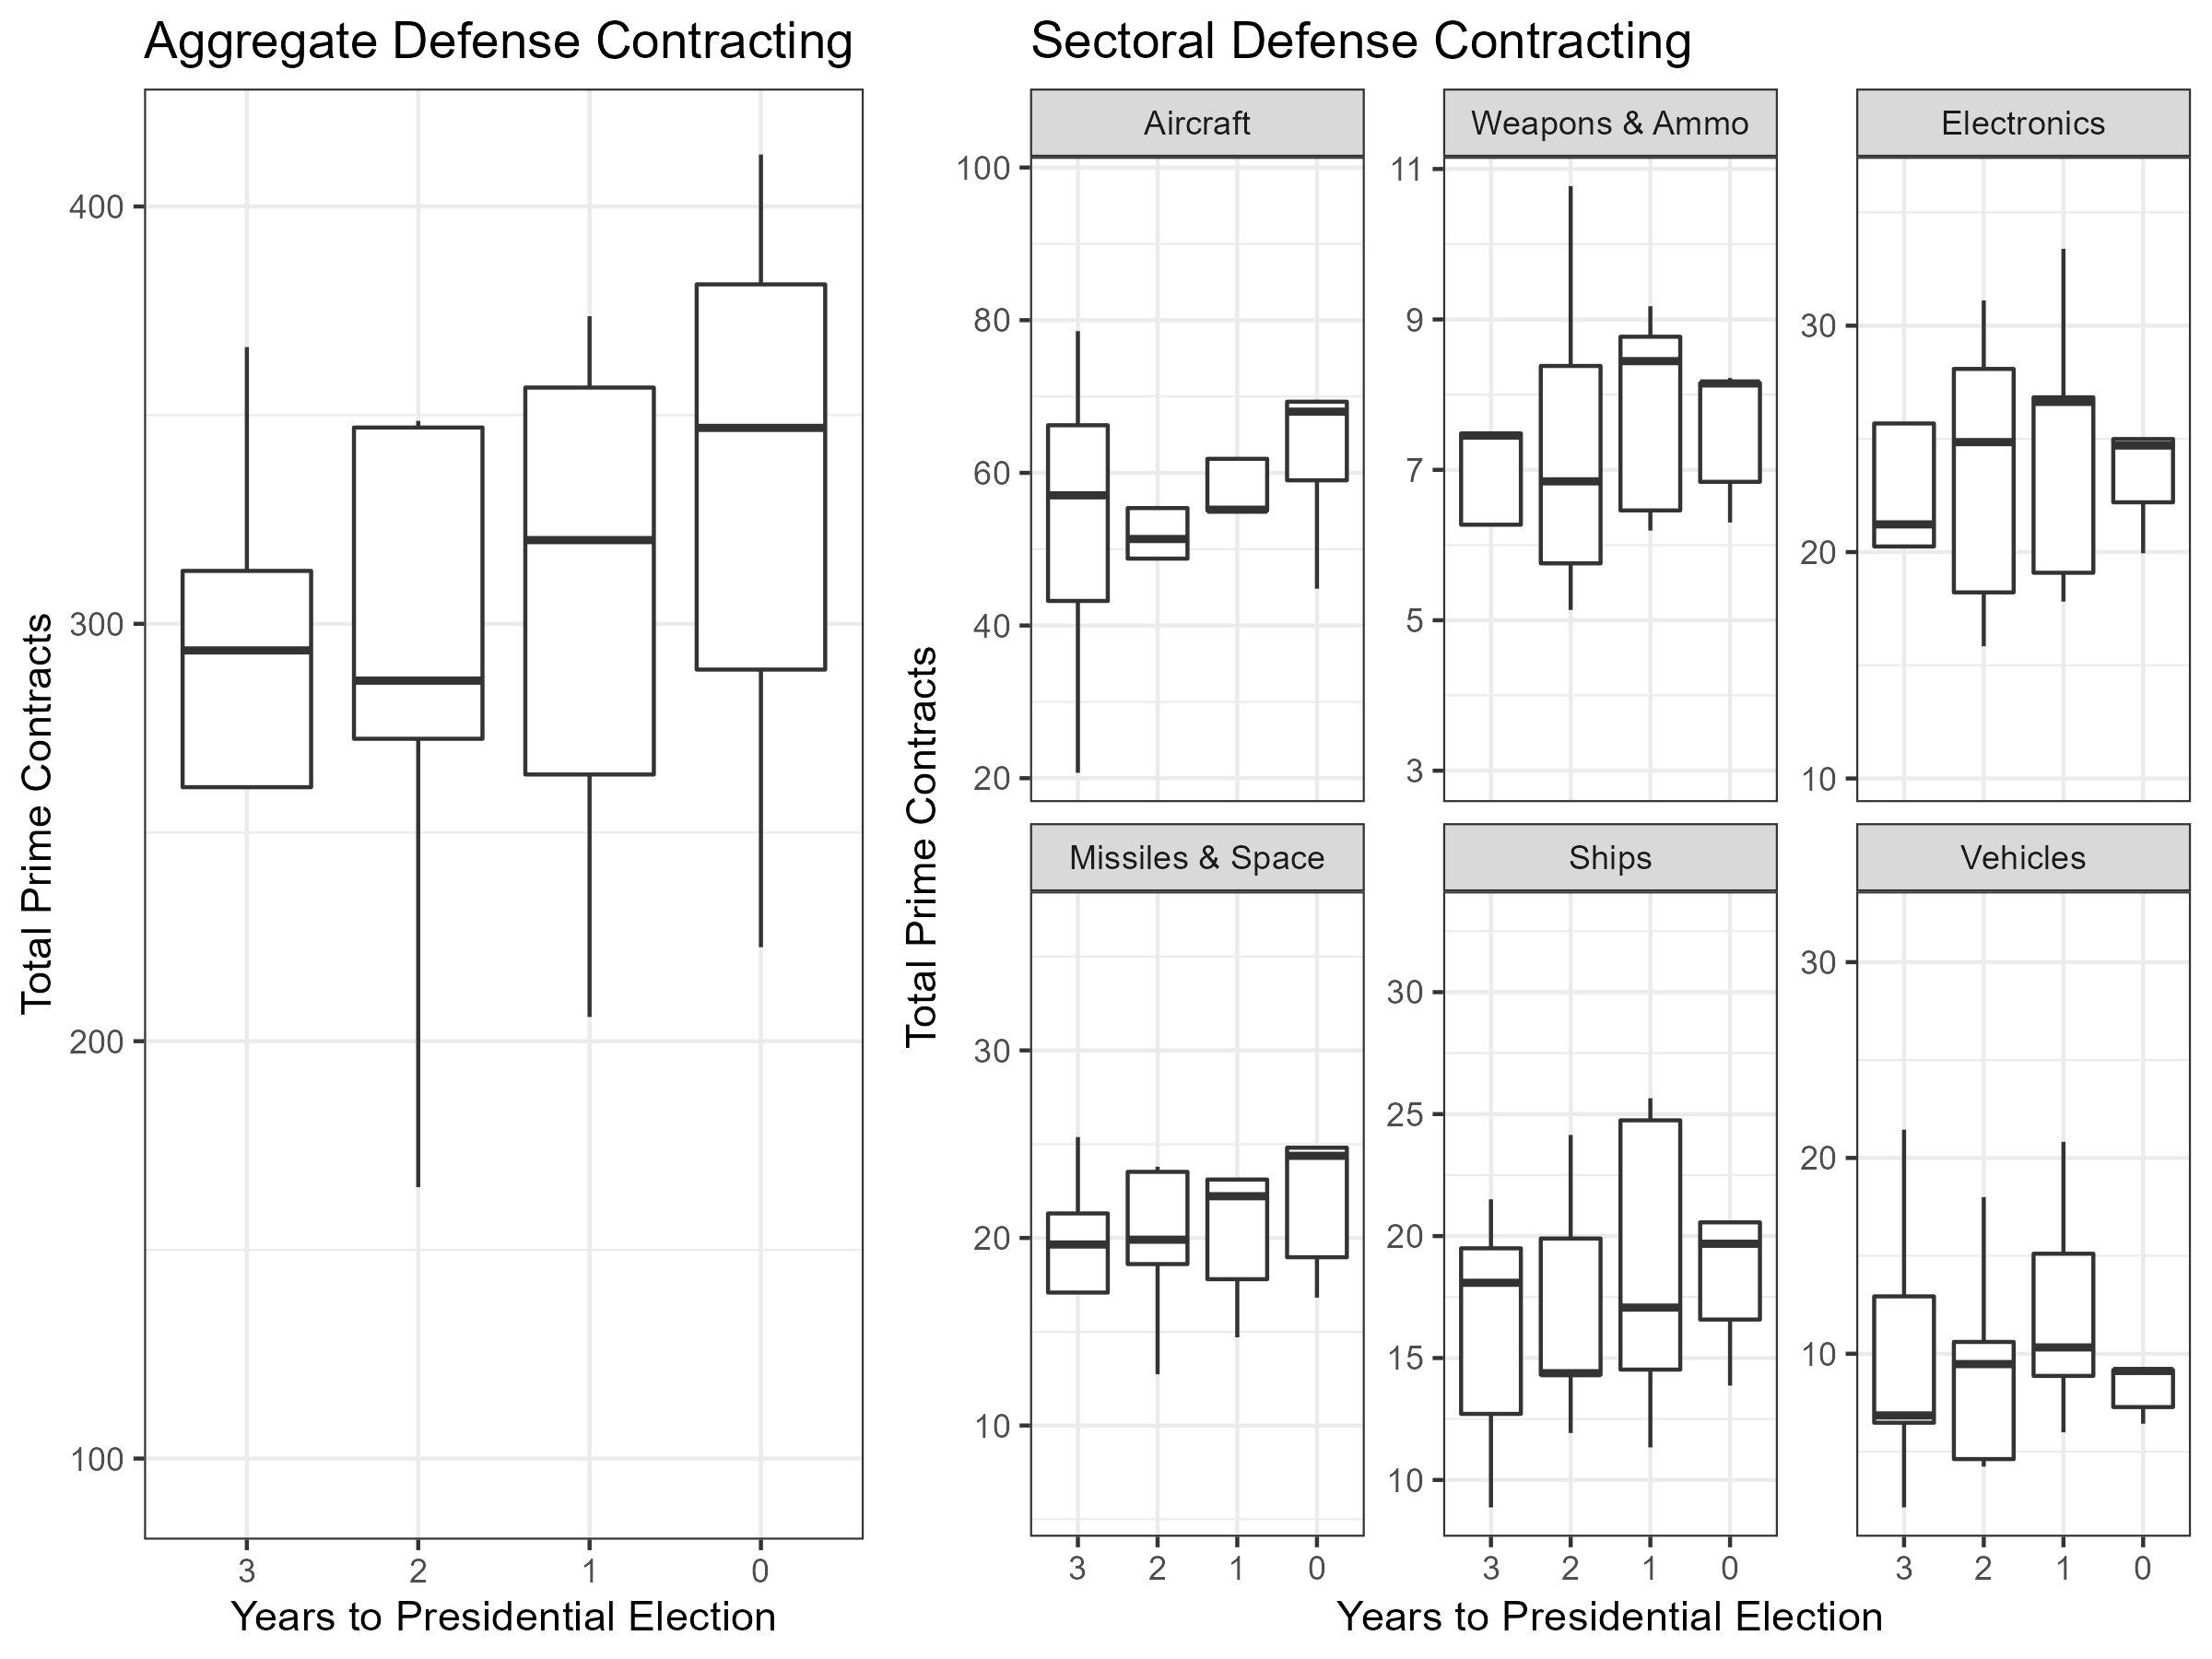
\includegraphics[width=0.95\textwidth]{../figures/contract-cycles.png}
	\caption{Distribution of prime defense contract awards by presidential election proximity, 2000-2020. The dark line in the box plot marks the median value of total contract awards in each year.}
	\label{fig:contract-cycles}
\end{figure}


Particular sectors drive the aggregate increase in defense contracting. 
Aircraft contracts increase dramatically, as do missile and space outlays. 
Naval contacts and prime awards for weapons and ammunition also increase, but retain a high level in the first year of many administrations, which changes those cycles. 
Electronics contracting also rise significantly, and there is a slight increase in vehicle contracting. 
Outside of aircraft, most of the specific platform cycles change the median contract outlay by less than \$10 billion.


Therefore, there is some evidence that defense contracting cycles follow presidential elections.
Along with prior research \citep{DerouenHeo2000}, this suggests that defense contracting is a plausible source of electoral cycles in arms exports from the United States to its allies.
Efforts to manipulate economic conditions through defense contracting have international ramifications. 


\section{Arms Transfers and Presidential Elections}


The next step in the argument suggests corresponding electoral cycles in U.S. arms deals. 
I model U.S. arms deals from 1951 to 2014 using deals data from the SIPRI Arms Transfer Database \citep{SIPRI2021}.
The outcome in this analysis is annual count of deals, based on SIPRI's trend indicator value methodology for major conventional weapons.
This section presents count data regression estimates of annual arms deals. 

% Why focus on deals
I analyze arms deals rather than observed arms transfers for three reasons.
First, elites can announce arms deals and related contracts immediately. 
Secondly, deliveries can take years after a deal is announced, even for second-hand or aid transfers of existing equipment. 
Finally, deliveries often space out the total value of a shipment over several years, especially for deals with many weapons or larger platforms. 


% models


\subsection{Results}


These results proceed in two parts.
First, I present the coefficient estimates from the Poisson regression. 
I then summarize the interaction of alliances and presidential election proximity in \autoref{fig:us-arms-plots}.


At the arms transfer hurdle stage, defense pacts increase the likelihood of any arms transfer, as does contiguity, shared IGO membership, and former colonial ties.
Increasing partner GDP increases the likelihood of arms transfers.
More distant states are also more likely to receive arms transfers, as the United States sells many arms outside the Western Hemisphere. 
After accounting for alliances, increasing democracy and U.S. GDP make arms transfers less likely, as did the Cold War. 
The negative Cold War coefficient reflects dispersion in U.S. arms transfers across more states after the USSR collapsed.


In the regression of arms transfer levels, states with a U.S. defense pact receive more arms in presidential election years. 
As with overall exports, the difference between allies and non-allies increases as time to an election decreases.
The key difference with the overall exports finding is that arms transfers to non-allies fall as presidential elections approach. 
This suggests that increasing exports from the United States to non-allies around elections concentrate in other goods. 


Alliances and elections are not the only meaningful predictors of arms deals.
Arms transfer levels are less sensitive to partner democracy, but increase with allied GDP and decrease with U.S. GDP. 
Contiguous, more distant and former colonial states also receive more transfers, as do states that share more IGO memberships with the United States.
The predicted probability of arms transfer coefficient implies that states that were more likely to receive arms are less likely to see large export increases.  
U.S. GDP growth reduces arms exports. 
The Cold War coefficient is largely negative, perhaps as the scale of arms transfers was more limited in that period. 
Last, there is some temporal autocorrelation in arms transfers, as the lagged dependent variable of .61 shows.


Again, the coefficient estimates are imperfect indicators of how alliances and electoral proximity interact.
\autoref{fig:us-arms-plots} therefore plots predicted arms transfers and marginal effect of defense pacts.
These predicted changes in arms transfers and estimated marginal effect of defensive alliances are consistent with the arms exports hypothesis.


\begin{figure}[htpb]
	\centering
		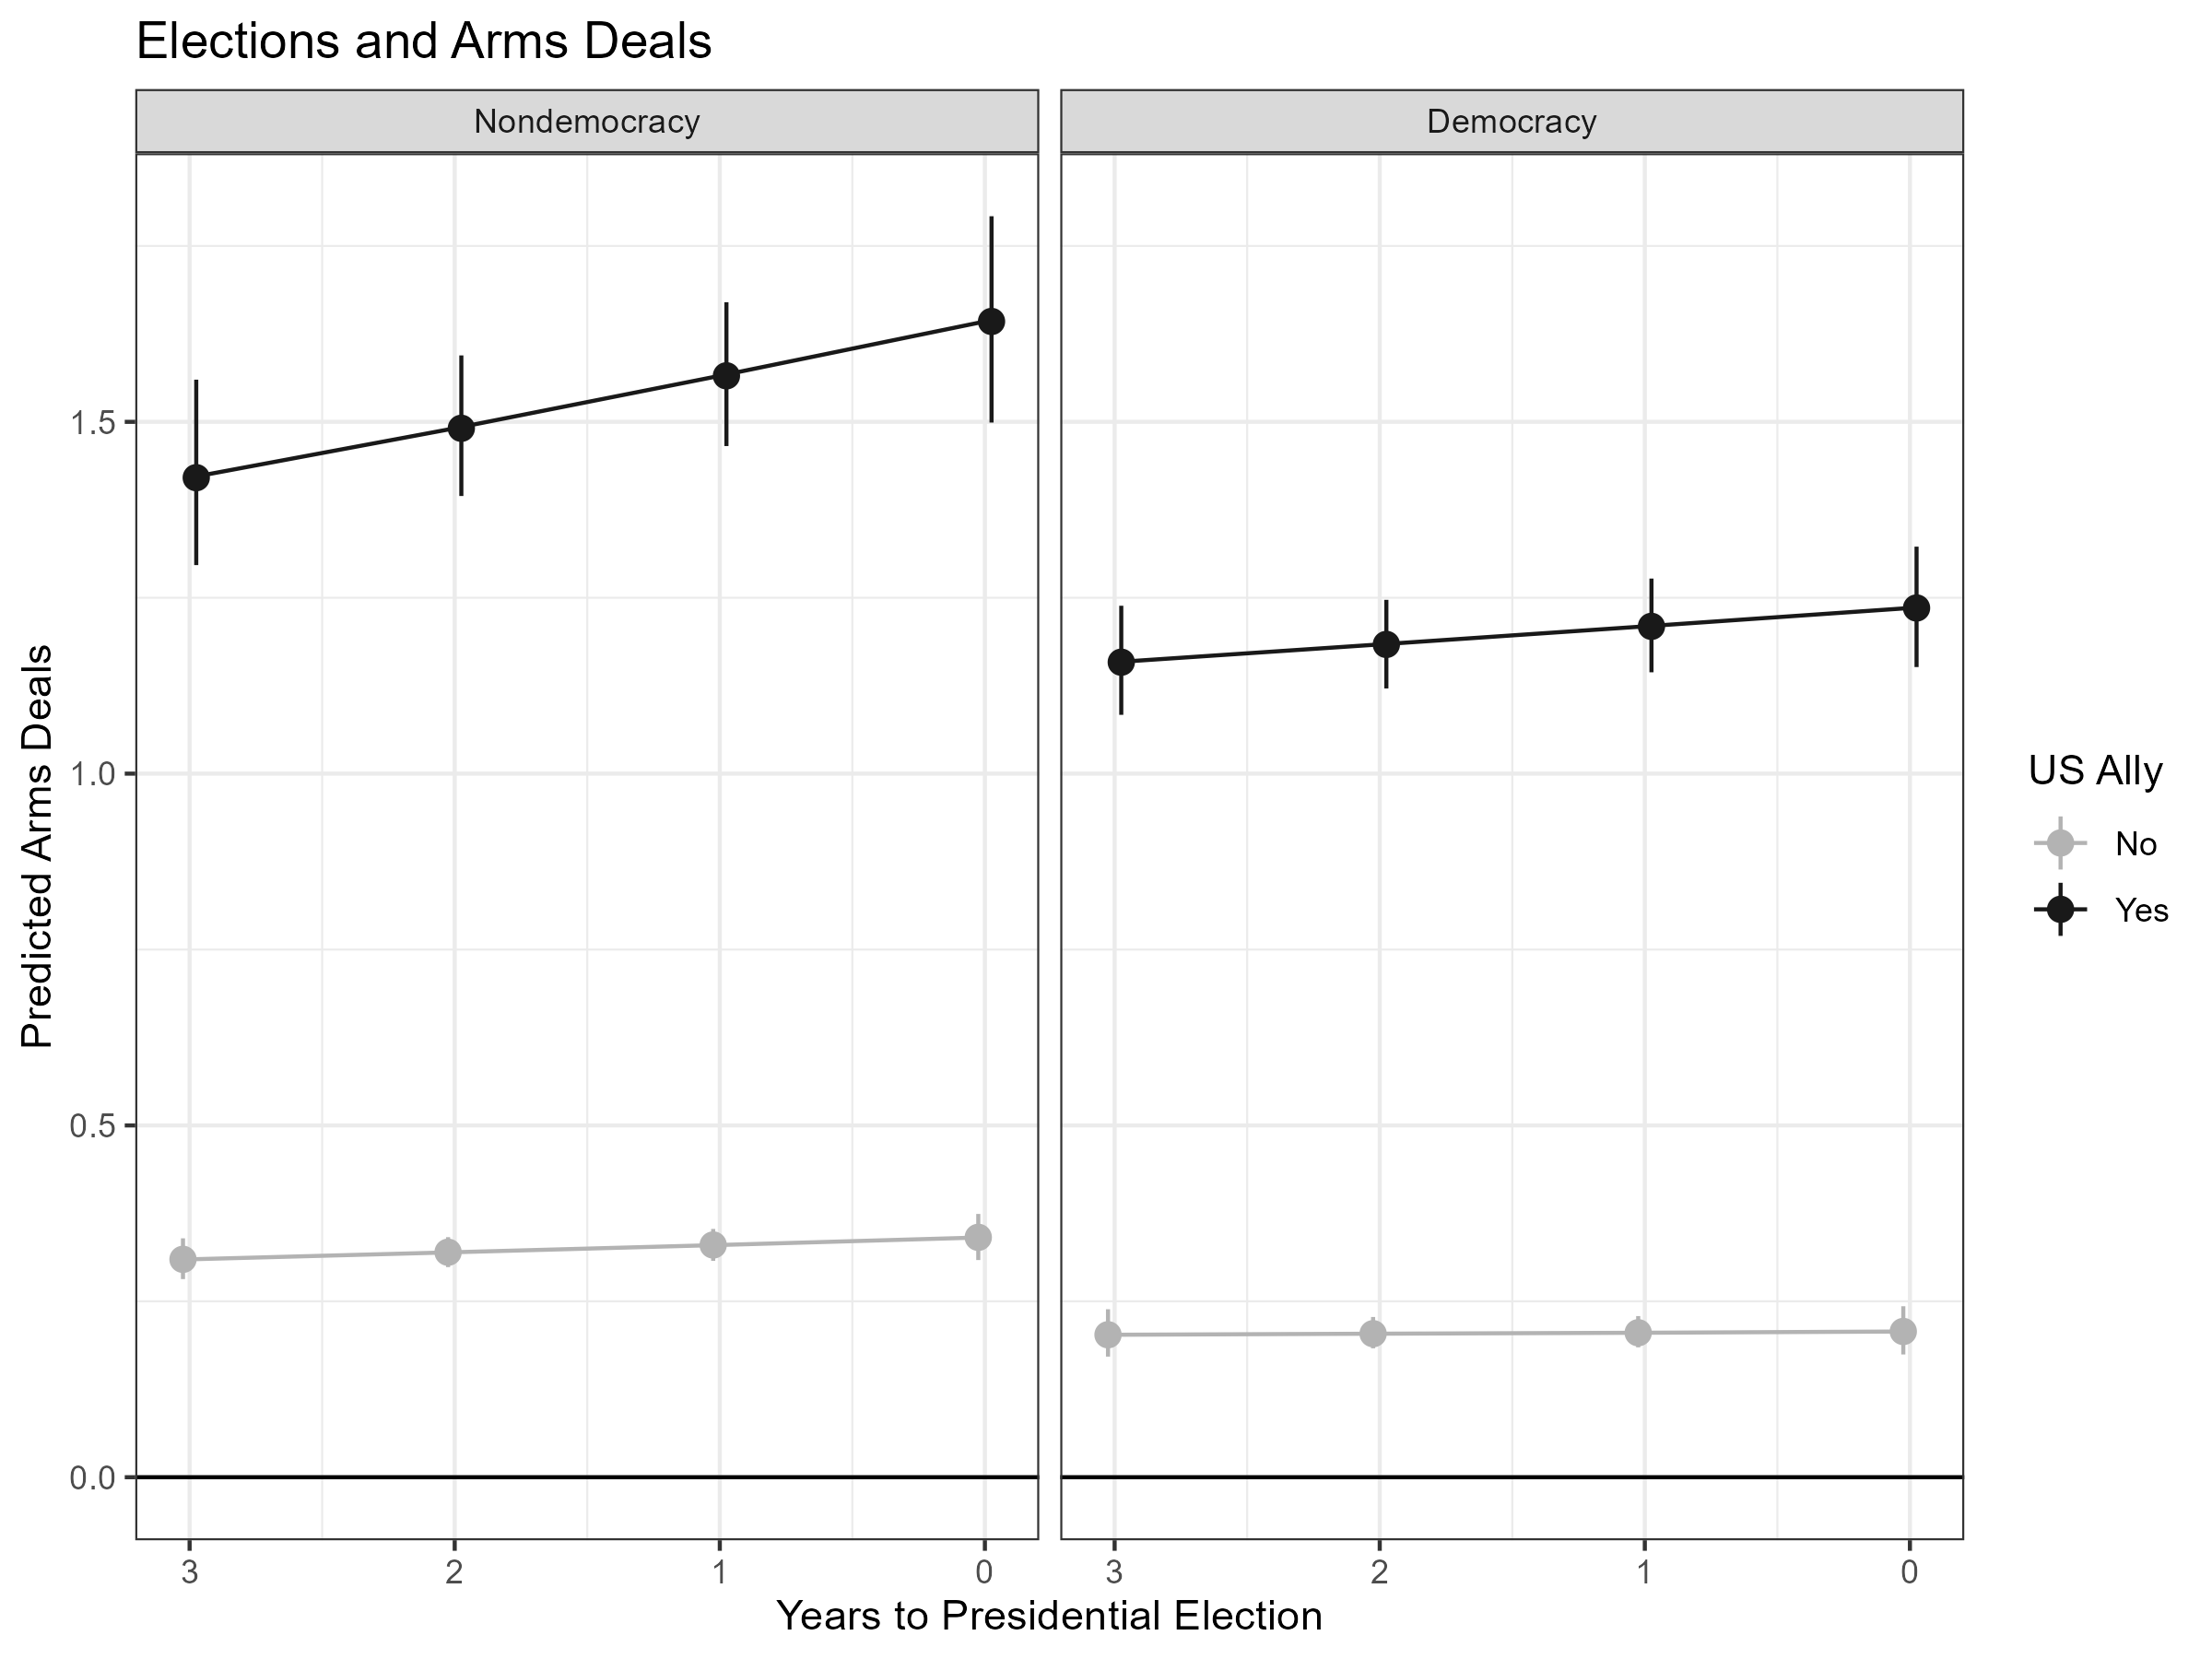
\includegraphics[width=0.95\textwidth]{../figures/us-arms-plots.png}
	\caption{Predicted outcome and the marginal impact of defensive alliances on changes in the log of arms transfers between the United States and other states 1950 to 2014. Points mark the estimates and error bars summarize the 95\% confidence interval.}
	\label{fig:us-arms-plots}
\end{figure}


First, predicted arms transfers to U.S. allies increase as presidential elections approach.
For a U.S. ally, predicted log arms transfers rise by .14 in expectation. 
This is roughly equal to the marginal effect of an alliance on overall exports reflected in \autoref{fig:us-elec-pred}.
At the same time, arms transfers to non-allies fall as elections approach. 


As a result, while arms transfers to allies and non-allies are similar in the year after a presidential election, there is a expected gap of .34 between allies and non-allies in election years.
The marginal impact of a defense pact on arms transfers reflects this difference, as it rises near presidential elections.
U.S. allies thus receive more arms near presidential elections than other states, as security cooperation and defense industry integration encourage arms exports.


Divergent electoral cycles in arms transfers reflect distinct political relations.
Allies have more to gain from accommodating electoral cycles in arms transfers, and can fit additional U.S. arms into military forces that already use U.S. kit.
Arms transfers cement cooperative relationships and bolster allied security through additional capability.
Leaders may also face more scrutiny over arms transfers outside alliances as elections approach. 


These growing arms exports to allies near elections are the result of electoral cycles in defense contracting. 
The next analysis unifies the defense contracting and arms deal models. 




\section{A Bayesian Model of Contracts, Arms Exports, and Trade}


The three individual analyses provide initial support for the argument, but they also treat each part of the process in isolation. 
To show the full process, I employ a generative model where each stage of the process informs the next level.
This move 
I employ this approach because standard multiple-equation models in political science cannot easily accommodate divergent levels of analysis.
Flexible structure and Bayesian estimation can capture a wide variety of complex data-generating structures, subject to careful model validation \citep{Betancourt2021}. 





\section{Discussion and Conclusion}


The argument and results suggest that political budget and defense contracting cycles expand international trade, especially arms exports to U.S. allies. 
Economic efforts to bolster presidential electoral prospects have international consequences. 
Additional goods from defense contracting cycles produce arms flows outside the United States.
This bolsters cooperative relations between the United States and its allies.


Allied economic and security statecraft thus helps U.S. leaders win elections. 
While this is not a part of formal alliance bargains, these informal linkages are essential to grand bargains between alliance patrons and prot{\'e}g{\'e}s.
Allies need not undertake these cycles deliberately, but their accepting arms transfers is part of a cooperative bundle of ties regardless.


Allied support for political budget cycles affects democratic alliance credibility and maintenance. 
A stable alliance bargain can develop if leaders anticipate the electoral benefits of defense contracting cycles and arms exports to allies.
When leaders expect that maintaining security commitment will have electoral rewards, they will be more likely to invest in alliances. 


These findings also add an international security component to the political budget cycle literature.
Alliance partnerships can allow leaders to manipulate economic conditions for electoral gain. 
By providing an outlet for defense contracting , allies help leaders contract for new goods with less attention to the absorptive capacity and force planning of the U.S. military.


Finally, the argument and findings add to prior findings that states manipulate international economic and security cooperation to bolster or undermine leaders. 
To give one example, \citet{ChyzhUrbatsch2021} show that Chinese soy tariffs reduced support for Republicans in the 2018 midterm elections. 
Allies have both motive and means to use economic and security cooperation to help leaders. 
Rather than undermine leaders, allied arms import decisions create positive inducements for regular cooperation.


Future research could proceed in several directions. 
First, cycles in other economic outcomes such as foreign direct investment, are an interesting area for study. 
Exploring the role of defense industry integration and intermediate goods in these arms cycles is also critical.
Whether these results generalize to autocratic alliances or other democratic alliance patrons is another worthwhile inquiry. 
Security partners of other alliance patrons may take similar actions in different industries, for instance.


In conclusion, political budget cycles reshape international economic and security cooperation.
Budget cycles increase trade and arms transfers to U.S. allies through economic growth and defense contracting.
Security cooperation can therefore facilitate electoral benefits for leaders. 


\newpage
\singlespace
 
\bibliography{../../MasterBibliography} 


\end{document}